\section{Description of the data sets}

The input features for all molecules in the data set were 512-bit Morgan circular fingerprints\cite{Rogers_2010}, calculated with a bond radius of 2, and derived from the canonical smiles, implemented in the RDkit\cite{rdkit}.

\textbf{Harvard Clean Energy Project}:The Clean Energy Project is the world's largest materials high-throughput virtual screening effort\cite{hachmann_lead_2014,hachmann_harvard_2011}, and has scanned more than 3.5 million molecules to find those with high power conversion efficiency (PCE) using quantum-chemical techniques, taking over 30,000 years of CPU time. The target value within this dataset is the power conversion efficiency (PCE), which is calculated for the 2.3 million publicly released molecules, using the Scharber model\cite{scharber_design_2006} and frontier orbitals calculated at the BP86\cite{perdew_density-functional_1986,becke_densityfunctional_1993}\/def2-SVP\cite{weigend_balanced_2005} level of theory.


\textbf{Dose-Response Data Set}:These data sets were obtained from the NCI-cancer database\cite{_nci_}.  The dose-response target value has a potential range of -100 to 100, and reports a percentage cell growth relative to a no-drug control.  Thus, a value of +40 would correspond to a 60\% growth inhibition and a value of -40 would correspond to 40\% lethality.  Molecules with a positive value for the dose-response are known as inhibitors, molecules with a score less than 0 return a cytotoxic effect. Results against the NCI-H23 cell line was taken against a constant log(concentration) of -8.00M and where multiple identical conditions were present in the data, an average was used.  It should be noted that for this data set, we assert smaller values represent a more desirable outcome. 


\textbf{Malaria Data Set}:The Malaria data set was taken from the \textit{P. falciparum} whole cell screening derived by combining the GSK TCAMS data set, the Novatis-GNF Malaria Box data set and the St Jude's Research Hospital data set, as released through the Medicines for Malaria Venture website \cite{23798988}.  The target is the EC50 value, which is defined as the concentration of the drug which gives half maximal response.  Much like the Dose response set, this is a minimization problem; the lower the concentration, the more potent the drug.

\subsection{Data Set Analysis via Dimensionality Reduction with Neural Networks - Information Landscapes}
When analyzing data sets for qualities such as diversity, it is important to make the distance measure consistent with the predictive model.  For example, if the prediction were made with a Gaussian process, it would be wise to use the distance model built into the kernel to analyze the diversity of the datasets studied.  This becomes somewhat more complex when the predictive method does not have a well defined distance measure built into it, such as a neural network.  Simply analyzing the diversity of the inputs through the use of a Tanimoto distance histogram, for example, is potentially a dangerous path since it does not acknowledge the highly connected nature of the neurons in a neural network.  We instead utilize an alternative measure, in which a neural network itself is used to compress the data into a resonable number of dimensions,~\cite{hinton_reducing_2006} upon which a visual inspection can reveal the diversity of the dataset.

This is achieved through training an unsupervised neural network, of which the loss function of each layer is determined by how well the output matches that of the previous layer.  Through sequential reduction in the number of neurons, the principle components of an input signal are amplified, and can be sampled.  To fine tune the weights of this neural network, the funneling architecture is mirrored, and the weights adjusted so that a loss function comparing the input and output of the network is minimized.  
\begin{figure}[h!]
\centering
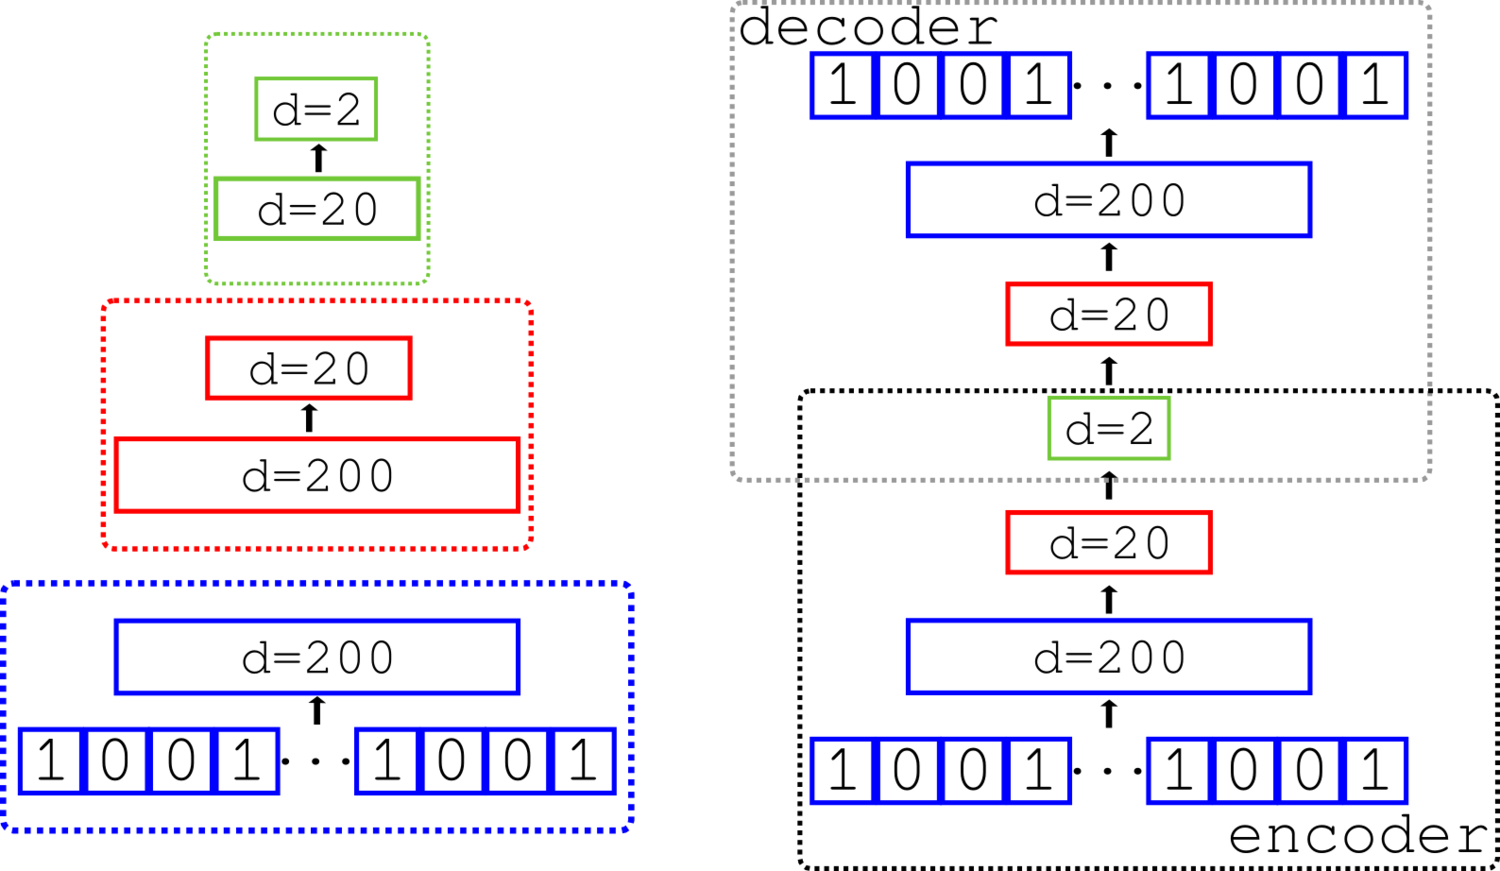
\includegraphics[width=1\columnwidth]{figures/nnet_decomp.png}
\caption{Neural networks can be used to compress data into a few, representative directions. In order to properly condition the weights of the neural network to be close to an optimal solution, the weights of each layer are pre-trained so that the layer reproduces the output of the previous layer (left).  These layers are then stacked into a funnel first decreasing in size (the encoder) and then increasing in size (the decoder).  Finally, the weights are fine-tuned to minimize reconstruction error (right).}
\label{fig:nn_decomp}
\end{figure}
The distributions of these network derived principle components were further investigated through the calculation of pairwise component distances. These distances were normalized so that the maximum distance was set at 1.0, and the minimum set to be 0.0. It can be seen from Figure \ref{fig:dist_hists}, that all of the sets are reasonably diverse in the eyes of the neural network.  As seen from figure 3, these sets are reasonably diverse in the eyes of the neural network. This statement may be counterintuitive from the chemical perspective, as perhaps one can think that molecules to carry out a specific task are likely to be more chemically similar. Global diversity measures can often give a misleading view into how models work on data. These measures can be thought of as a map of the local surroundings in chemical space.  To extend the metaphor, if you are looking to find the best place for a picnic, it is more helpful to have a streetmap than a globe.
  
  

\begin{figure}[h!]
\centering
\includegraphics[width=1\columnwidth]{figures/NN_distances_all/NN_distances_all.png}
\caption{The distribution of pairwise component distances, as calculated through the neural-network based procedure.  The distances were normalized to be in the range 0 to 1, where 1 is the maximal distance between two sets of components.  The histogram (top) was set to contain 100 bins, and is complemented below by a violin plot, in which the 25th, 50th and 75th percentiles are marked.  A violin plot is similar to a box-plot, but its width at any point is derived from a kernel density estimate of the underlying data.}
\label{fig:dist_hists}
\end{figure}

The underlying information derived from these network derived components can be further investigated through the use of a plot we call an 'information landscape'.  In this plot, chemical space (as described by the components, which are bound between 0 and 1) is split into areas of size 0.2x0.2 arbitrary units. The mean value for the targets contained within each area is calculated, and determines the color of that area.  In order to visualize the distribution of molecules within this depiction of chemical space, a kernel density estimate is used to plot contour lines.  Additionally, the top 100 molecules, ranked according to their target value, are plotted as points on the surface.  By analyzing the distribution of the data, alongside the location of extreme molecules, it is easy to classify the data into types of information landscape.  In Figure \ref{fig:info_landscapes}, we can see the information landscapes created to describe each of the data sets used within this study.  The Clean Energy Project dataset is striking in the strength of the input/property relationship --- the majority of the top molecules are concentrated in a relatively small area of chemical space.  Additionally, in this dataset, there is a clear trend for worsening performance as the Y-axis is ascended.  This is not the case for the other two datasets, in which the `good' areas of chemical space are more randomly distributed.  It is interesting to observe the One-Dose data set, in which there are two clear families of extreme molecules, one towards the top of the plot and one towards the bottom left.  This could be indicative of two different approaches taken in the literature to approach the problem of developing good treatments for this particular type of cancer. 
\begin{figure}[htb]
\centering
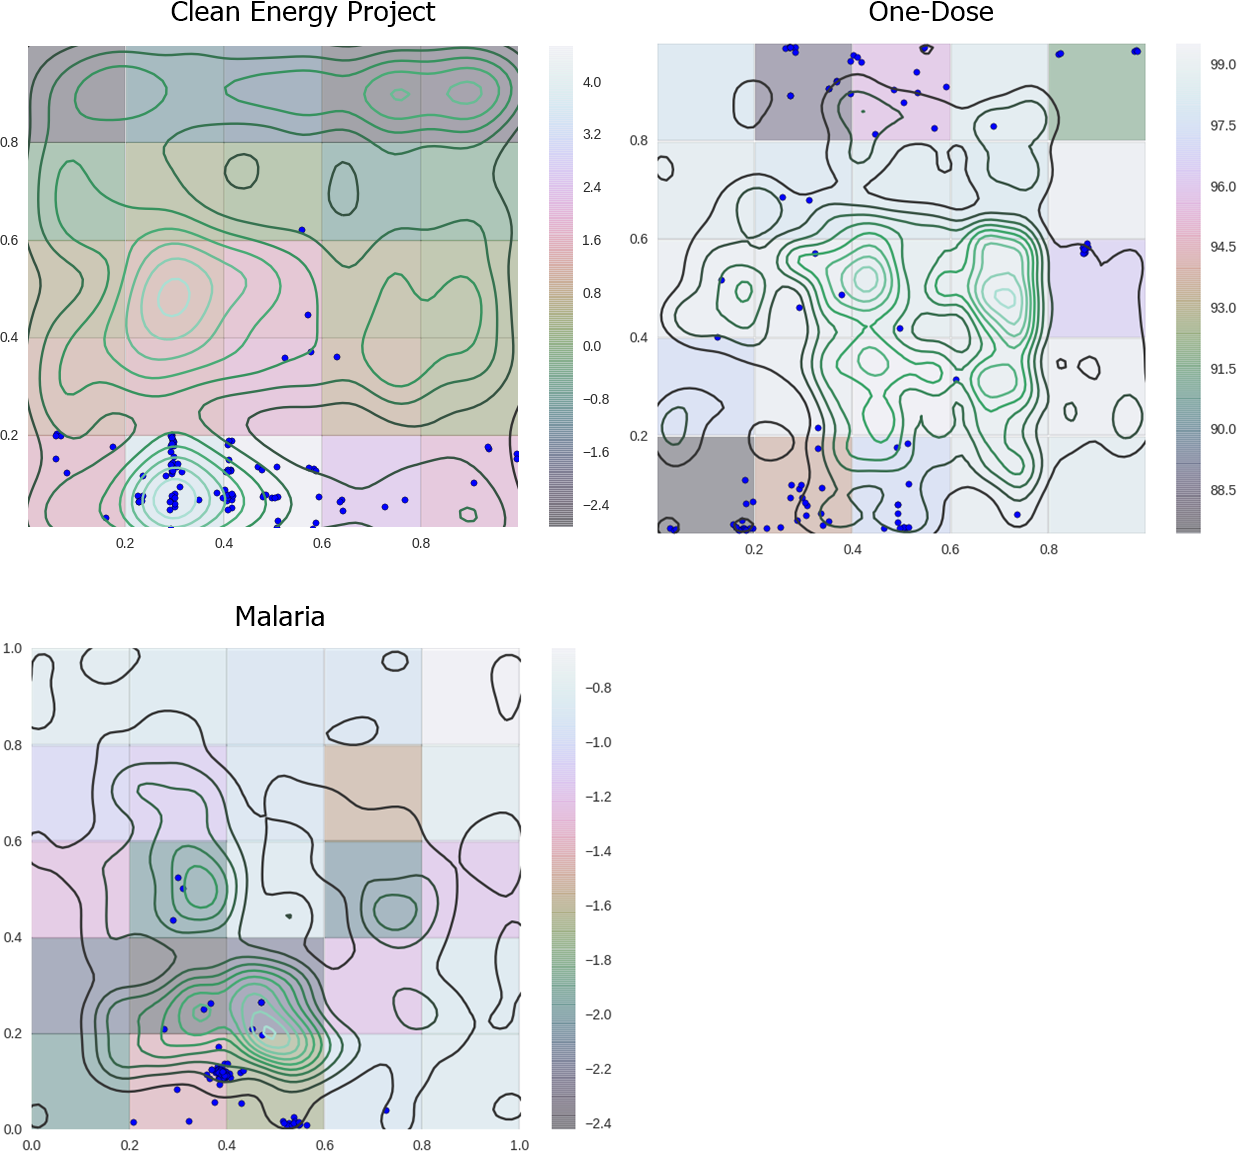
\includegraphics[width=\columnwidth]{figures/info_landscape-tile/info_landscape-tile.png}
\caption{Information landscapes for the Clean Energy Project, One-Dose and Malaria datasets.  The colors represent the mean value of targets whose reduced dimensional inputs fall within that area of reduced feature space, the contour lines are a kernel density estimate of the location of inputs, and the blue dots represent the location of the reduced dimensional features which represent the top 100 target values for each set.}
\label{fig:info_landscapes}
\end{figure}
